\documentclass{article}
\usepackage[a4paper, top=2cm, bottom=2cm, left=2cm, right=2cm]{geometry}
\usepackage{tikz}
\usetikzlibrary{calc, positioning, shapes.misc, fit}

\pagestyle{empty}

\begin{document}
	\begin{center}
		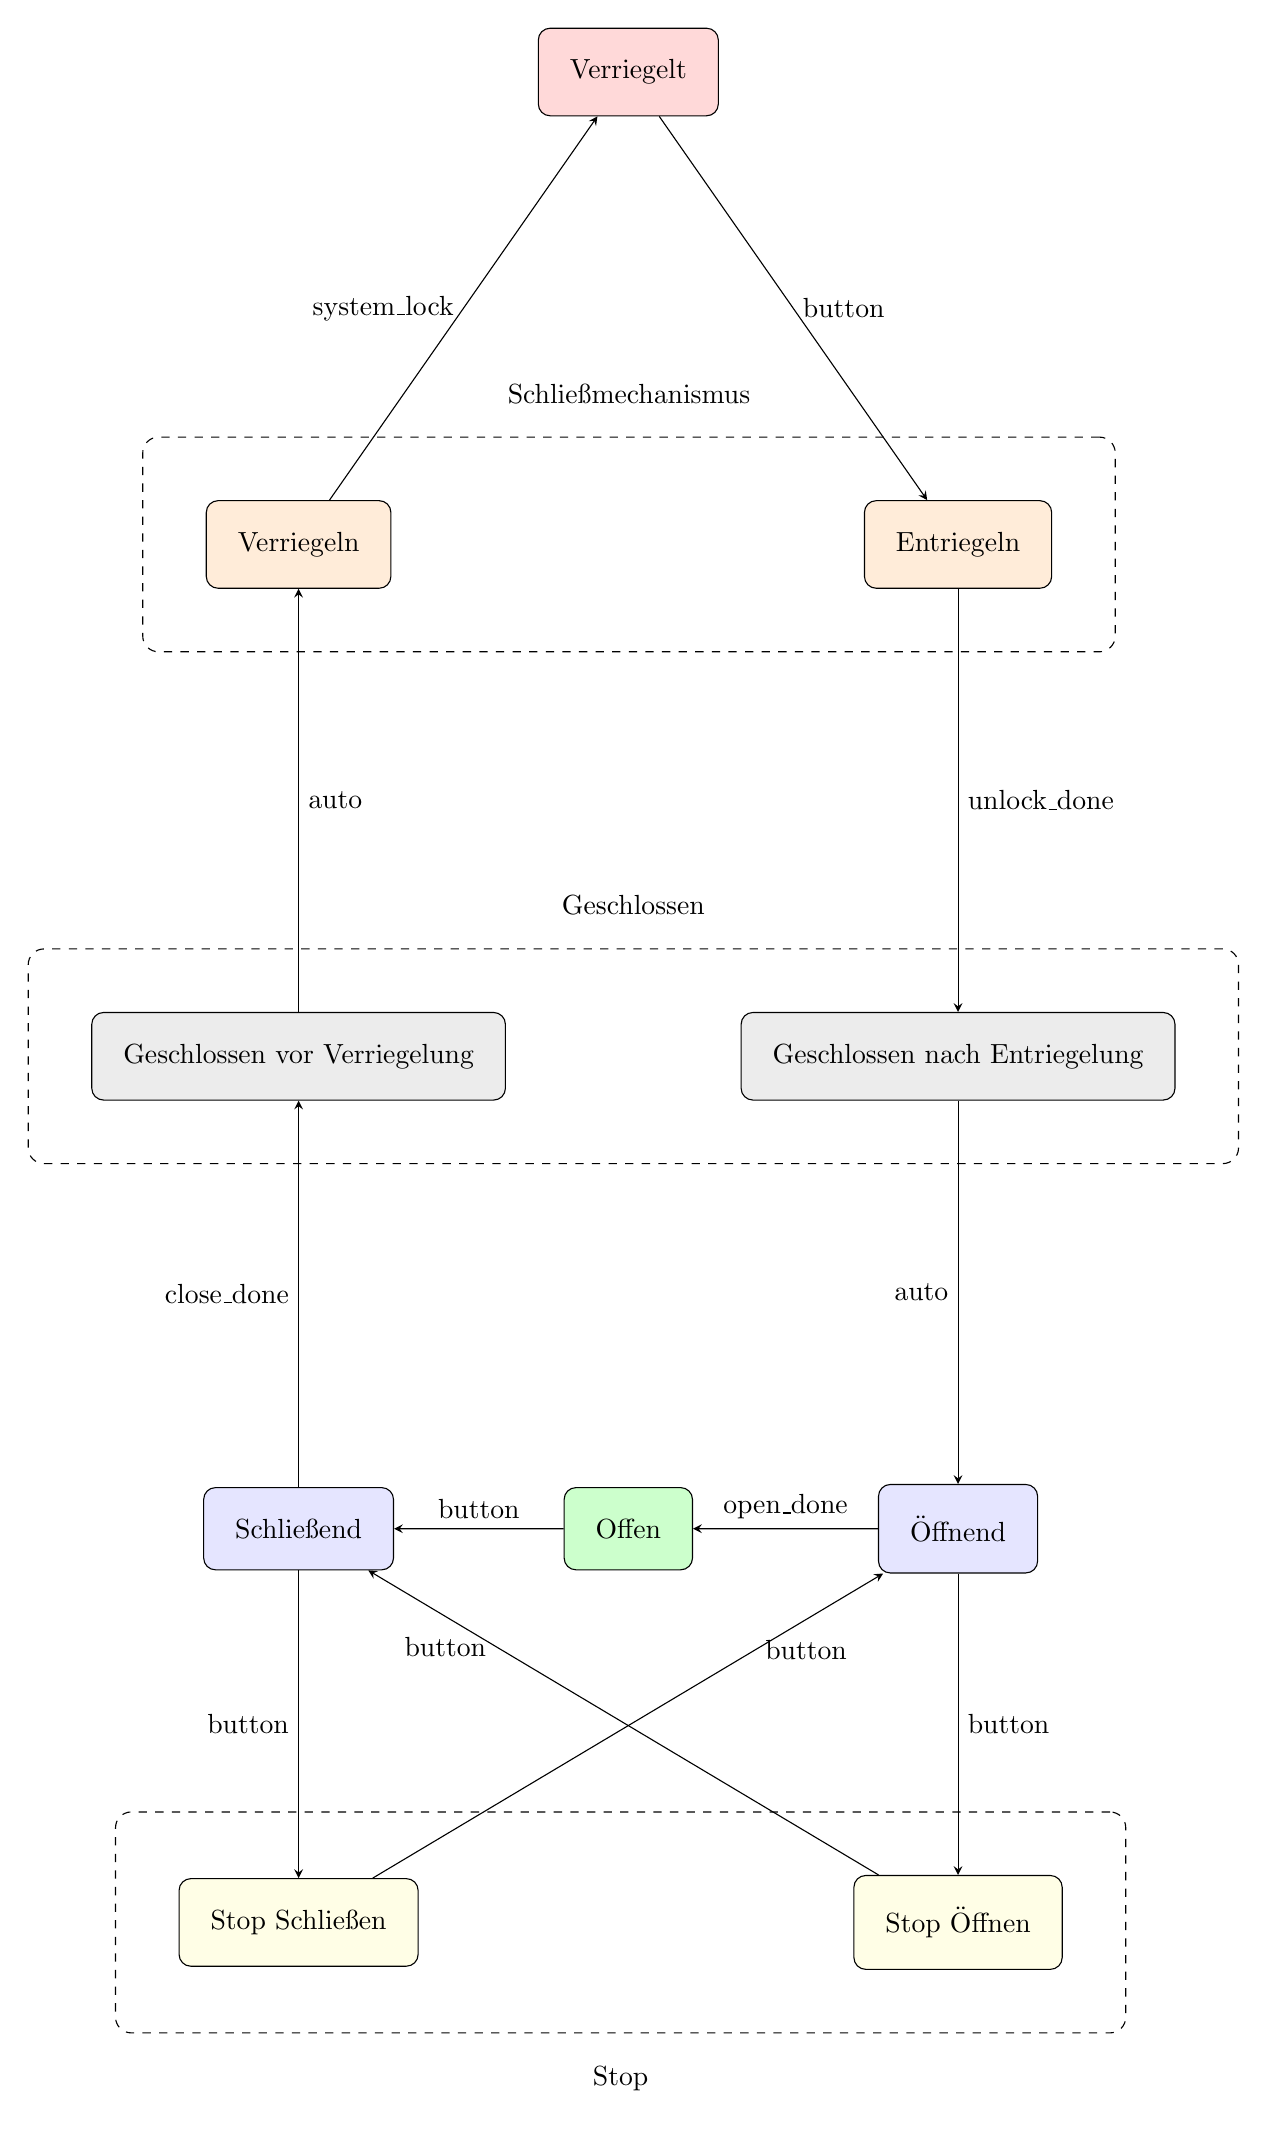
\begin{tikzpicture}[
			round/.style={rounded corners=1.5mm, inner sep=4mm, draw, align=center, node distance=5cm},
			every node/.style={font=\normalsize},
			->, >=stealth,
			]
			
			% Hauptzustände
			\node[round, fill=orange!15] (Verriegeln) at (0,4) {Verriegeln};  
			\node[round, fill=orange!15, right=6cm of Verriegeln] (Entriegeln) {Entriegeln};
			\node[round, fill=red!15] (Verriegelt) at ($(Verriegeln)!0.5!(Entriegeln)+(0,6)$) {Verriegelt};
			\node[round, fill=gray!15] (GeschlossenL) at ($(Verriegeln)+(0,-6.5)$) {Geschlossen vor Verriegelung}; % Links unter Verriegeln
			\node[round, fill=gray!15] (GeschlossenR) at ($(Entriegeln)+(0,-6.5)$) {Geschlossen nach Entriegelung}; % Rechts unter Entriegeln
			\node[round, fill=blue!10] (Schließend) at ($(GeschlossenL)+(0,-6)$) {Schließend};
			\node[round, fill=blue!10] (Öffnend) at ($(GeschlossenR)+(0,-6)$) {Öffnend};
			\node[round, fill=green!20] (Offen) at ($(Schließend)!0.5!(Öffnend)$) {Offen};
			\node[round, fill=yellow!10] (StopSchließend) at ($(Schließend)+(0,-5)$) {Stop Schließen};
			\node[round, fill=yellow!10] (StopÖffnend) at ($(Öffnend)+(0,-5)$) {Stop Öffnen};
			\node[draw, dashed, rounded corners=2mm, inner sep=8mm, fit=(StopSchließend)(StopÖffnend), 
			label={[label distance=3mm]below:{Stop}}] {};
			\node[draw, dashed, rounded corners=2mm, inner sep=8mm, fit=(Entriegeln)(Verriegeln), 
			label={[label distance=3mm]above:{Schließmechanismus}}] {};
			\node[draw, dashed, rounded corners=2mm, inner sep=8mm, fit=(GeschlossenL)(GeschlossenR),
			label={[label distance=3mm]above:{Geschlossen}}] {};
			
			
			% Transitionen
			\path
			(Verriegelt) edge node[right] {button} (Entriegeln)
			(Entriegeln) edge node[right] {unlock\_done} (GeschlossenR)
			(GeschlossenR) edge node[left] {auto} (Öffnend)
			(GeschlossenL) edge node[right] {auto} (Verriegeln)
			(Verriegeln) edge node[left] {system\_lock} (Verriegelt)
			(Öffnend) edge node[above] {open\_done} (Offen)
			(Öffnend) edge node[right] {button} (StopÖffnend)
			(StopÖffnend) edge node[near end, left] {button} (Schließend)
			(Schließend) edge node[left] {close\_done} (GeschlossenL)
			(Schließend) edge node[left] {button} (StopSchließend)
			(StopSchließend) edge node[near end, right] {button} (Öffnend)
			(Offen) edge node[above] {button} (Schließend)
			;
			
		\end{tikzpicture}
	\end{center}
\end{document}
